\section{Procedure And Methods}
\subsection{System Architecture}
\begin{figure*}
	\begin{center}
		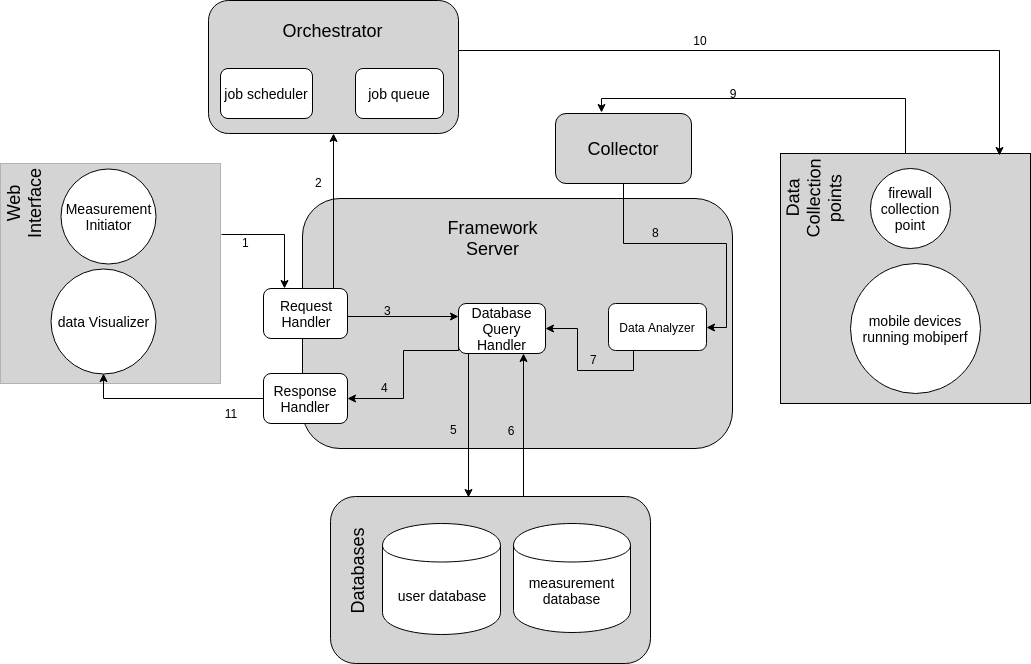
\includegraphics[width=1\linewidth]{res/system.png}
	\end{center}
	\caption{Showing the system overview, different components making the system and the communication directions between these components in the systems.}
	\label{figure:system}
\end{figure*}
Figure ~\ref{figure:system} shows the system over, the components of the system and how everything will fit together. The lines from components are communication lines and suggest the communication direction between the comments. 
\paragraph{}
Following is a mapping for each of the line number and the communication information that is sent via that line:
\begin{enumerate}
	\item  This is the request to the request handler to decide to send it to the query handler or the orchestrator.
	\item This is the message sent to the orchestrator to data collection.
	\item Database query sent from request handler to the database to get data from the database.
	\item Data returned from the database to the response handler.
	\item Database query sent  to the database to the query handler to retrieve data.
	\item Data returned from the database to the query handler.
	\item Results of data analysed by the analyser.
	\item Data sent from the collector to the data analyser..
	\item Data returned from the data collection points to the collector.
	\item Request sent from the orchestrator to the collection points to initiate collection of data.
	\item This is the response sent from the response handler to the data visualizer to display the data obtained from the database.
	
	\end{enumerate}
The components of the system as seen from the figure ~\ref{figure:system} are:
\paragraph{\textit{Framework Server}}
This is the base of the application. Other components like the orchestrator and the Collector rely on the server. The server provides communication to the database system, it also provides a means for scheduling measurements requested via the orchestrator as well as keeping track and ensuring that the jobs are sent to the collector for starting. It also consists of other tools like the request handler which is the communication point from the web interface. Lastly it provided a component for handling the logic for communicating with the Databases. The reason for having only one central point for database communication is so that if we decided to change the database used, the only part of the system that needs to be modified is just this component. We also have a response handler which handles and sends results from the database to users that they are associated with in the web interface. Lastly, we will have an analyser of he network data which receives the data from the collector and performs analysis and then saves the data in the database. This part is where the machine learning algorithms can be implemented for making decisions and also adding more jobs on the scheduler.

\paragraph{\textit{Web Interface}}
This consists of the Measurement initiator and the Visualizer tool. From this the users are able to view the network activities in form of graphs. The users are able to also view their profiles which will also be indicated by the visualizer. The measurement initiator is a tool for researchers who want to run network measurements on the network.

\paragraph{\textit{Orchestrator and Collector}}
These are the two services that run on top of the framework server. They are responsible for accepting requests from researchers as well as initiating measurements form phones and collecting data from probes.

\paragraph{\textit{Data Collection points}} This consists mobile phones running a Mobiperf extended application. These are where we are measuring the network measurements that will be displayed by the visualizer.
\paragraph{\textit{Database}} Made up of two separate databases for storing measurement data and the other for storing user data.
\subsubsection{Measurement Orchestration}
In terms of orchestration, once measurements are scheduled a job will be stored on the web server with information on the measurement experiment to be run based on user-defined fields such as a number of nodes as well as parameters to measure.When the scheduled time is reached, the Server will send push notifications to online nodes with information on what parameters to be measured. Once the data is collected it will be sent to the measurement database.
\subsubsection{Network Measurement Collectors}
We need to develop a phone application that will be the means of collecting measurements for the internet metrics. We have decided to build an android application for the phones and tablets as Android is open and requires less resources to get started. According to \cite{statcounter_global_stats}, Android currently has 35\% of the operating systems market. This shows how popular amongst users android is and thus will be a good platform to consider to build the application for first. 
\paragraph{}
The application that we will be building will be extending the MobiPerf application which is built in Java \cite{m-lab}. Since Android Development is also done in Java it also adds to why we will be focusing on developing for android as it is easier to extend an already existing platform compared to creating one form the beginning. The mobile phone are the mobile clients shown on Figure 1. These clients will be talking to the HTTP server to send data to the database or to be triggered to collect network measurements.
\subsubsection{Visualizer}
To design the visualizer, a co-design process will adopted. During the co-design process, about three workshops  will be conducted. A number of users from the Ocean View community will be invited to take part in these workshops. Different Human Computer Interaction methods will be employed to achieve the desired user experience. These will involve both end users and the team taking part in designing and come up with ideas. Co-design is sometimes called participatory design which is defined by \cite{ctx2100202260004041} as a set of theories,practices and studies related to end-users as full participants in activities leading to software products. Thus the reason why we adopted this method as we want to involve users in the design process.
\paragraph{}
The  Django python web framework will be used to build a visualizer web app from the ground up. The framework will be used to implement an HTTP server that will query data from either database1 or database2 as shown on the system design. Data will then be exposed in the form of API endpoints to a front end web framework that will display data in the form of graphs.
\paragraph{}
The advantage of choosing the Django web framework is that it is a simple framework that is easy to use and comes with most back-end functionalities already implemented \cite{10.1007/978-3-540-87403-4_11}. Django also has a lot of support in the Python community, which makes it a reliable option for this project.
\paragraph{}
For the front end, the web app will leverage the react.js a JavaScript front end web framework to build user-friendly interfaces. React is a component-based library which allows rapid prototyping of web applications\cite{Gackenheimer2015}. It also managed by Facebook hence making it a reliable and trustworthy tool to use.
